\chapter{Background and Related Work}
\label{chap_background}

% background

% social robots 
% - what makes social robots work
% - social model
% - what has been done in social robots

% empathy
% - what is empathy?
% - why do we feel empathy
% - what are the different kinds of empathy
% - which empathy matters?

% backstories
% - do backstories increase empathy?
% - 

%This work sits at the intersection of empathy and social robotics. 


\section{Social Robotics}
This work falls under the field of social robotics. Breazeal defined social robots as autonomous robots that are explicitly designed to encourage people to apply a social model to interact with them \cite{breazeal_social_robots}.

We are inherently social creatures. To survive and function as a group, we have evolved to understand the intent, desiress and beliefs of other individuals \cite{lieberman_social}. However, our ability to ascribe mental states to others tends to overgeneralize to non-human and even non-living entities. Hieder and Simmel found that when presented with a complex animation of geometric shapes, people projected intentions and emotions on to them. For sufficiently complex artifacts, where we cannot explain their behavior by simple laws of physics or by our understanding of their design, thinking of the artifacts as agents with intention provides us with some predictive powers \cite{dennett_intentional_stance}. Nass et al. showed that given a minimal social cues, people tend to treat computers as they would treat social others \cite{nass_media_equation}. In one study, Nass found that when asked to rate a computer on how well it performed a task, participants rated the computer more highly when they did the rating on the same machine versus on a different computer. This seemingly polite treatment occurred even if the rater was technically competent. Braitenberg showed that we anthropomorphize even simple robots with perceived goals and autonomy \cite{braitenberg_vehicles}.  Our willingness to apply social model to certain innanimate objects makes social robots possible. 

% An important goal for social robotics is to be able to design innanimate objects so that they encourage the use of social model in our interaction with them.  A central question for design is the issue of believability. ie how does the non-living create a perception of life \cite{bates_believability}? A key part of the answer is motion. The animators at Walt Disney who authored the Illusion of Life came up with principles of motion that convey life, techniques which Pixar brought to 3d animation \cite{lasseter_computer_animation} As an example of the application of these principles, consider Luxo Jr, Pixar's iconic table lamp (Figure \ref{pixar_luxo_jr}). Even though it is insistently inorganic in form, through motion it creates a perception of life-likeness. Designers of social robots have taken inspiration from the work of digital animators and designed robots that are organic and expressive in their motion \cite{hoffman_robot_movement}.  

   \begin{figure}[thpb]
      \centering
      \includegraphics[width=3in]{figures/intro/pixar_luxo_jr.png}
      \caption{Pixar's Luxo Jr. showing squash-stretch animation \cite{lasseter_computer_animation}}
      \label{pixar_luxo_jr}
   \end{figure}


An important goal for social robotics is to be able to design innanimate objects so that they encourage the use of social models in our interaction with them.  A central question for design is the issue of believability, that is, how does the non-living create a perception of life? \cite{bates_believability} A key part of the answer is motion. The animators of Walt Disney understood this well; through expressive movement, they could turn a faceless carpet into a believable character on screen. The principles of animation that Disney pioneered were brought to 3d animation by Pixar \cite{lasseter_computer_animation}. As an example of these principles, consider Luxo Jr., Pixar's iconic table lamp (Figure \ref{pixar_luxo_jr}). Composed of rigid linkages, the lamp is insistently inorganic in form, yet through squashing and stretching its apparent size it creates a perception of life-likeness and can convey emotional states. Social roboticists have taken inspiration from the work of digital animators and designed robots that are organic and expressive with their movement \cite{hoffman_robot_movement}.  

% \begin{figure}[htbp!]
% \begin{center}
% %\framebox[\textwidth][l]{
% \includegraphics[width=1.0\textwidth]{figure/pixar_luxo_jr.png}
% %}
% \end{center}
% \caption{{\it Pixar's Luxo Jr. showing squash stretch animation technique \cite{lasseter_computer_animation}}
% \label{pixar_luxo_jr}}
% \end{figure}

% TODO add something about contingent action

For the appearance of the robot, social robotics has experimented with a wide range of forms, ranging from a simple wheeled robots to a human-like form. Paradoxically, forms too close to human can seem eerie \cite{mori_uncanny_valley}. Many successful social robots are designed to resemble creatures or cartoonish human figures. Leonardo, which resembles a fantastic gremlin, is an example of zoomorphic robot. Creature like appearance or juvenile features result in low expectations of interaction, making people more forgiving of mistakes that a robot might make. In addition to form and motion, the field has uncovered many other design principles that make robots more socially evocative including emotional expression, human oriented perception, and non-verbal communication to name a few \cite{fong_survey_socially_interactive_bots}. I draw on these successful principles for the design and behavior of the zoomorphic robot presented in chapter 4. The main contribution of this work is a design principle for behavior, creating and communicating an implicit life-story, that could aid in the design of emotionally engaging robots. 

% TODO add something about applications of social robot




% cynthia-q: do I justify my work in this section?
\section{Empathy}
\label{sec_background_empathy}
Empathy comes from the german word Einf\"{u}hlung or ``in feeling'' which was used to describe the ability to project one's personality into a perceived object \cite{empathy_etymology}. Empathy is now widely used to describe the ability of feeling and understanding another - usually humans - experience as our own \cite{decety_human_empathy}.

De Waal traced the evolutionary origin of empathy to the need for a mother to rapidly understand the emotional state of her offspring \cite{de_waal_altruism_empathy}. Once the empathic capability was developed, the trait was used for broader social relationship. The evolutionary argument suggests that empathy is influenced by a perceived similarity between a subject and target, and empirical evidence supports this view \cite{krebs_empathy_altruism}.

How do we understand the experiences of another? As discussed above, we have an innate ability to attribute mental states of beliefs, desires and intentions to others, an ability referred to as Theory of Mind (ToM) \cite{frith_social_cognition}. Simulation theory, which offers one basis for ToM, contends that we use our imagination to put ourselves in another's place and use our mind to simulate theirs. To the question of what someone else wants or feels, we ask ourselves what would our mental state be if we were in that individual's situation. Goldman argues that this pretension of being the other leads to empathy: ``The initial pretend states are then operated upon by psychological processes, which generate feelings, attitudes, or affects that are similar to, or homologous to the target individual's states'' \cite{goldman_empathy_mind_morals}. It stands to reason that if we are engaged by a social robot that we perceive to have a mind, and we use our own experiences to understand those of the robot, we would feel empathy towards it. 

Advent of neuro-imaging techniques has shed light on the neural pathways responsible for empathy. Lieberman describes two neural mechanisms that work in conjunction to help us understand the experiences of the other: a mirror system that we recruit to understand \emph{how} someone is performing a task, and a mentalizing system that let us understand \emph{why} they are doing so \cite{lieberman_social}. Lieberman identifies two additional neural processes that are implicated in empathy: an affect matching system which allows us to feel what the other feels and an empathic motivation system, located in the septal area, that rewards us for helping another. 

% tying empathy to simulation theory
% central cases of empathy, so construed, may arise from simulation, that is, from
% imaginatively adopting the perspective of another. such initial `pretend' states are tehn operated upon by
% psychological processes, which generate feelings, attitudes, or affects that are similar to, or homologous to,
% the target individual's states. Furthermore, just as the simulator is generally aware of his
% states as simulations of the target, so the empathizer is presumed to be aware of his vicarious affects and
% emotions as representatives of the afefcts and emotions of the target.\cite{goldman_empathy_mind_morals}
%
% In summary, from our evidence, we suggest that both, ToM and empathy, depend on the activation of similar brain networks involved in social perception, namely the mPFC, superior temporal lobe and temporal pole. These areas form the basis for making inferences about the mental states of others. However, the appreciation of the other’s emotional states requires the additional engagement of emotional networks, particularly the amydgala. \cite{vollm_fmri_empathy}


%Empathy or the capacity to "put oneself in other's shoes" is widely regarded as an important pro-social trait \cite{eisenberg_empathy_prosocial}.  So it stands to reason that if a subject were to use their own stories to perceive the experience of another, they would find the target's experience to be similar to their own and consequently would be in a position to feel empathy for the target.

% TODO NEUROLOGICAL account

Psychologists broadly categorize empathy into affective and cognitive empathy. Affective empathy involves feeling what other feels while cognitive empathy has to do with understanding another's point of view. Davis operationalized the definition of empathy with the Interpersonal Reactivity Index (IRI), a now widely used scale for measuring trait empathy \cite{davis_multidimensional_empathy}. In the IRI, Davis distinguished four kinds of empathy as follows: Fantasy, Perspective Taking, Empathic Concern and Personal Distress; the former two represent cognitive empathy and the latter two, affective empathy. The Fantasy scale measures tendency to identify with imagined characters such as those in fiction or movies. Perspective Taking scale guages the tendency to spotaneously adapt the viewpoint of another. Empathic Concern measures tendency to feel concern or sympathy for an unfortunate other. Personal Distress scale captures tendency to feel personal anxiety when witnessing others in difficult situation. In this project I use the operationalized definition, the IRI scale, for measuring empathy. The particular subscales that show greatest effect in my studies will help shed light on the nature of empathy that people feel for robots with life-stories. 




\section{Robots and Empathy}

% TODO: slater? 

Empathy interaction with robots has recently been studied. Leite et al. investigated the effect of empathic behavior of a robot towards a human. They found that a robot making empathic statements towards a human based on their state of gameplay in a chess match was rated as more companionable than a robot producing neutral statements \cite{leite_empathic_chess_robot}. In this work, the direction of empathy studied is reversed: I am exploring human empathy towards robots. 

Rosenthal Von der Putten et al. showed videos of tortured robots to participants and measured their emotional arousal and ttrait empathy using the IRI. Participants were negatively affected by the experiment and expressed empathy for the robot \cite{rosenthal_emotional_reaction}. The validation study in my thesis uses negative treatment of robots inspired by this study and others to test for empathy towards robots \cite{bartneck_daisy_daisy} \cite{verbunt_mockingbird_robot}. A key difference, howerver, is that this thesis tests a new design crteria for encouraging empathy, namely implicit life stories. Reik et al. found that more anthropomorphic a robot is, the greater the empathy the robot evokes supporting the idea that empathy is mediated by perceived similiarity and this extends to artificial agents. If self-similiarity increases empathy, augmenting a robot's experience using our own should also increase empathy. Seo et al. showed that embodiment matters: a physical robot invokes greater empathy than a 
virtual agent showing the same behavior \cite{seo_empathy_virtual_physical}. In this latter study, the robot pretended to malfunction to elicit empathy . Among other effects, as part of the malfunction, the robot lost its memory. While the study was not about testing effect of loss of memory, I find the result to be encouraging for my thesis. 


% Attachment to robots

%  - Nass -> anthropomorphize. we project life-like qualities on to computers. 
%  - Fong -> design for emotionally engaging robots.


%  We consider robots to be life-like



\section{Artificial Agents and Stories}

% We attach emotional value to objects with back-stories . Walker and Glenn conducted an informal experiment where they bought ordinary objects such as ashtrays and teacups from eBay and then resold them with a fictional story about the object. For instance, the ashtray was resold with a story saying that it was given to the seller by his dying grandfather. These objects sold for a higher price than the purchase. This result is encouraging. What distinguishes my work from this project is that the robot is not a passive participant in the world but is perceived to be experiencing the world;the life-story is not about the robot but of the robot. 

The effect of stories on perception of objects was explored by the Significant Objects Project \cite{walker_significant_objects}. Walker and Glenn claimed that the emotional value of an ordinary object was increased when it was presented with a story of some signficance attached to it. An important distinction between this project and my proposed work is that the stories were about the object and not of the object. The objects did not purport to be transformed by the experience; rather they had events happen to them. A robot on the other hand, can be perceived to have a mental state and thus have its own story.

Research has shown that entities with perceived agency are more engaging when given a backstory. Bickmore et al. created a virtual agent exercise coach that made up a fictitious human autobiography from fragments of handcrafted story-lines. For instance, the agent could say that her parents used to take her hiking and camping. Although the virtual agent was incapable of having such a story, the researchers found that participants talked more frequently with such an agent than with one without a backstory \cite{bickmore_virtual_agent_autobiography}. Similarly, Gockley et al. designed a robot receptionist with an evolving human storyline to keep visitors engaged with it. Valerie, the robot receptionist, talked to visitors about her singing career and social life using stories written by dramatists. As the stories unfolded over an year, some visitors interacted with her regularly to follow the narrative \cite{gockley_valerie_roboreceptionist}. 

Even without human back-stories, robots that change in behavior over time can foster longer human interactions.  A long-term study at a kindergarten by Kanda et al. showed that a robot using pseudo-development can keep children interested in it when the novelty effect wears off \cite{kanda_long_term_robovie}. Toys like Tamagotchi have used pseudo-developement to emotionally engage users, although a user's attachment to the Tamagotchi can be partially attributed to the dependency of the Tamagotchi on the user \cite{kaplan_artificial_attachment}.

To my knowledge, the closest work to this thesis is Lee et al.'s investigation of the effect of cognitive development of a robot on its social perception \cite{lee_aibo_development_presence}. Lee showed that human participants who trained an AIBO to perform some preset tasks considered the robot to be more life-like and having a stronger social presence. While this result is encouraging, one key difference between the this thesis and Lee's is that I am interested in understanding the effect of development on perception of the robot even if there was no training investment on part of a participant. Investment, shared experience, dependency can be layered on, but in this work, I am interested in exploring whether a minimal life-story can evoke empathy.

Over the next few chapters, I will discuss the studies and robot designs that will test this thesis. 

% 4-6 4:45pm
% 4-7

